\chapter{Linear Algebra}
\label{ch:linalg}

\section{Products}
\subsection{Hadamard Product}
\subsection{Matrix Multiplication}
\subsection{Dot Product}
\subsection{Kronecker Product}
\subsection{Inner Product}
\subsection{Dot Product}

\section{Determinant}

\section{Eigen Vectors and Values}

\paragraph
Eigenvectors describe a transformation using the form: 

\[\displaystyle A\mathbf {u} =\lambda \mathbf {u}\]

$A$ is the transformation matrix, $\mathbf {u}$ is the eigenvector, and $\lambda$ is the eigenvalue.

It is useful to think about eigenvectors visually\footfullcite{3b1beigen}. Consider a modern 2d image manipulation program.
These programs often have transform handles, usually little circles or squares that you can click on and drag
with your mouse in order to scale and squish and image. 

\begin{figure}[h]
\caption{Unwarped arrow with a slope of 1}
\centering
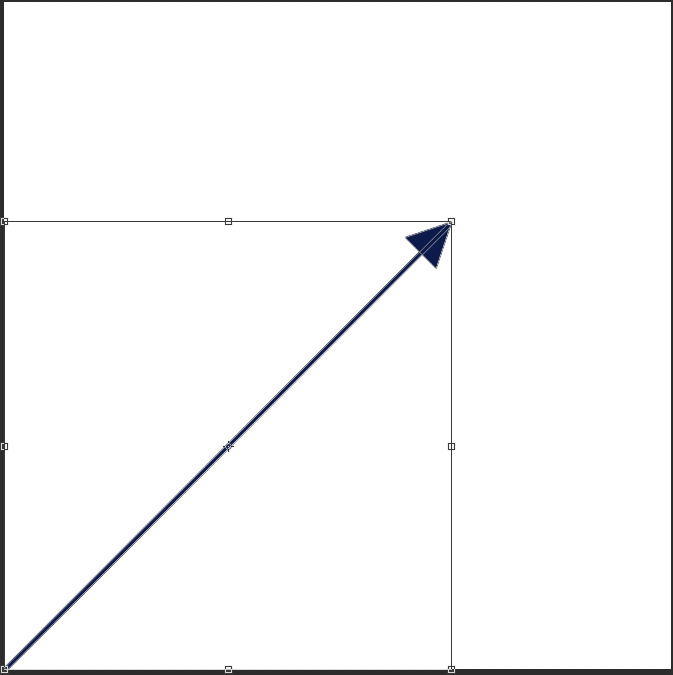
\includegraphics[width=0.25\textwidth]{unwarped_arrow}
\end{figure}

Consider what happens when you enlarge an image
in only the Y direction. The image becomes taller and warped. By skew I mean that an arrow starting from the 
bottom left of the image and extending to the top right of the image will no longer have the same slope. 

\begin{figure}[h]
\caption{Warped arrow with a slope greater than 1}
\centering
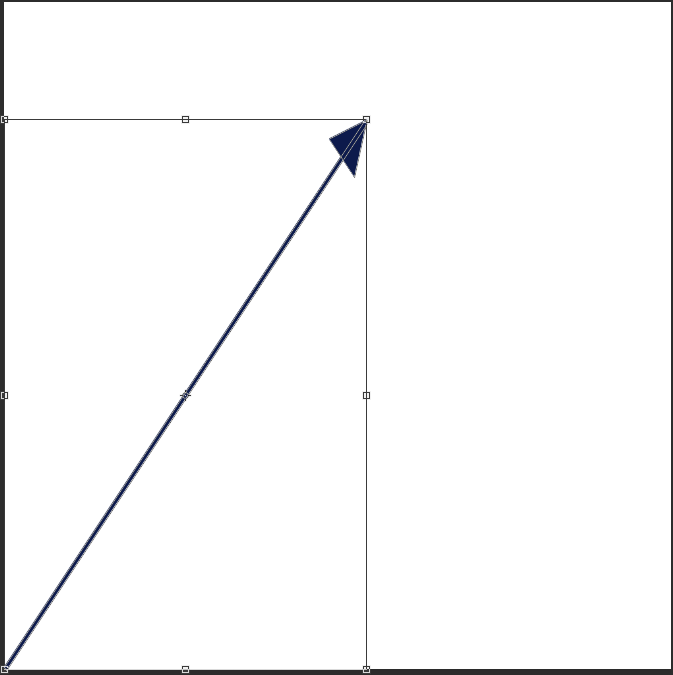
\includegraphics[width=0.25\textwidth]{warped_arrow}
\end{figure}

This makes intuitive sense. If we've literally dragged the tip of that arrow upwards so its slope (rise over run)
must increase as it is "rising" more than it used to while it is "run" is the same. 

The eigenvector is the direction in which we are performing this scaling and the eigenvalue is how much
we scale by.

Let's consider how we can calculate these values.

\[\displaystyle (A-\lambda I)\mathbf {u} =0\]

To make this equation true, $A-\lambda I$ should be a transformation that will take anything you give
it and squish it down to 0 volume. So in the 2 dimensional case, if we give the transformation a square
with area, lets say 9,
it should squish it (and anything else) down to a line with area 0. This concept of how much a transformation
scales volume is called the determinant. So the determinant of this transformation must equal 0.

We need to pick a $\lambda$ that we can subtract from each value on the diagonal of A such that
$det(A-\lambda I)=0$. There can be more than one or they can even be imaginary! In the case where you have a 
complex eigenvalue, there is no corresponding eigenvector.

When considering rotation around an axis in three directions. The eigen vector is the axis and the eigenvalue
is 1. The eigenvalue is 1 because rotation does not scale.

\section{Distance functions}
\subsection{L1 and L2 distances}
The L2 distance is defined as:

$$\operatorname{L2}(\vec{x}, \vec{y}) = \sqrt{\sum_{i=0} (x_i - y_i)^2}$$

This is the euclidean distance. If you plot all the points around some point that have the same distance,
you will trace an n-sphere. An n-sphere is just the sphere representation in n dimensions. So an n-sphere
where $n=2$ will be a circle. 

\begin{figure}[h]
\caption{L2 distance}
\centering
\includegraphics[width=0.25\textwidth]{example-image}
\end{figure}


This has some nice properties, including rotational invariance, 
shift invariance and when scaled the relative distances remain the same. Contrast this with the L1 distance.

$$\operatorname{L1}(\vec{x}, \vec{y}) = \sum_{i=0} (|x_i - y_i|)$$

Which is commonly called the manhattan distance. While this function is shift invariant, and mantains
relationships when it is scalled, it is not rotationally invariant. 

To see this, lets do the same visualization as the L2 distance. If we plot all the points that are the same
distance away from some point we get a n-cube (square when $n=2$) with its corners on the axes instead of an
n-sphere. 

\begin{figure}[h]
\caption{L1 distance}
\centering
\includegraphics[width=0.25\textwidth]{example-image}
\end{figure}

When we rotate the coordiate axes, so that the corners of the n-cube rotate with it, all of the distances
change (assuming we are not rotating $\frac{\pi}{2}$ along an axis). 

Lets double back and define what it means to be shift invariant. 
$$= \sum _{i=1}^{n}|p_{i}-\mu-q_{i}+\mu|$$
$$= \sum _{i=1}^{n}|p_{i}-q_{i}+\mu-\mu|$$
$$= \sum _{i=1}^{n}|p_{i}-q_{i}|$$

Here $\mu$ is some constant that we are shifting all the points by. Notice that the constant
cancels out. The same is true for the L1 distance. 

Likewise for maintaining relationships after scaling
$$= \sum _{i=1}^{n}|\frac{p_{i}}{\sigma}-\frac{q_{i}}{\sigma}|$$
$$= \sum _{i=1}^{n}|\frac{1}{\sigma}(p_{i}-q_{i})|$$
$$= \frac{1}{\sigma}\sum _{i=1}^{n}|p_{i}-q_{i}|$$

\subsection{Computing the L2 distance efficiently}
\paragraph
While the L2 distance can be trivially computed using nested for loops,
we often have access to blazing fast linear algebra libraries that obviate 
this need. We can see massive speedups if we define our distances in terms
of the primitive computations that these libraries offer, namely matrix multiplication.

Now instead of a single $\vec{x}$ and $\vec{y}$ we have $X$ and $Y$ which are many
$\vec{x}$s zipped row wise, and the same for $\vec{y}$. 

To do this, lets take another look at our L2 distance.

$$\operatorname{L2}(X, Y) = \sqrt{\sum_{i=0} (X_i - Y_i)^2}$$

What happens if we expand $(X_i - Y_i)^2$?
Remeber that $(a-b)^2 = (a-b)(a-b) = a^2 - 2ab + b^2$. So:

$$\operatorname{L2}(X, Y) = \sqrt{\sum_{i=0} X_i^2 - 2X_i Y_i + Y_i^2}$$

Well $X^2$ is really just the element wise product of $X$ and itself. 
This is called the Hadamard product and is widely available in linear algebra
libraries. 
$$(A\circ B)_{ij}=(A\odot B)_{ij}=(A)_{ij}(B)_{ij}$$

The same applies to $Y$. 

So we can break out of the summation and just do:

$$\sqrt{\sum_{i=0}X \circ X + \sum_{i=0}Y \circ Y - 2(X \cdot Y^T)}$$
Which will give us a matrix where each element is the L2 distance between a row in $X$ and a row in $Y$

